\documentclass[a4paper,12pt]{article} 

% First, we usually want to set the margins of our document. For this we use the package geometry.
\usepackage[top = 2.5cm, bottom = 2.5cm, left = 2.5cm, right = 2.5cm]{geometry} 
\usepackage[T1]{fontenc}
\usepackage[utf8]{inputenc}

% The following two packages - multirow and booktabs - are needed to create nice looking tables.
\usepackage{multirow} % Multirow is for tables with multiple rows within one cell.
\usepackage{booktabs} % For even nicer tables.

% As we usually want to include some plots (.pdf files) we need a package for that.
\usepackage{graphicx} 

% The default setting of LaTeX is to indent new paragraphs. This is useful for articles. But not really nice for homework problem sets. The following command sets the indent to 0.
% \usepackage{setspace}
% \setlength{\parindent}{0in}
\usepackage{indentfirst}

% Package to place figures where you want them.
\usepackage{float}

% The fancyhdr package let's us create nice headers.
\usepackage{fancyhdr}

\usepackage{amsmath,amsthm}
\usepackage[most]{tcolorbox}


% To make our document nice we want a header and number the pages in the footer.

\pagestyle{fancy} % With this command we can customize the header style.

\fancyhf{} % This makes sure we do not have other information in our header or footer.

\lhead{\footnotesize Computer Organization(H): Final Review}% \lhead puts text in the top left corner. \footnotesize sets our font to a smaller size.

%\rhead works just like \lhead (you can also use \chead)
\rhead{\footnotesize Mengxuan Wu}

% Similar commands work for the footer (\lfoot, \cfoot and \rfoot).
% We want to put our page number in the center.
\cfoot{\footnotesize \thepage} 

\begin{document}

\newtcolorbox{tipsbox}{
  colback=yellow!20!white, % Background color
  colframe=blue!80!black,  % Border color
  fonttitle=\bfseries,     % Title font
  title=More Info,         % Box title
  breakable                % Make the box breakable
}

\newtcolorbox{warningbox}{
  colback=yellow!20!white, % Background color
  colframe=red!80!black,   % Border color
  fonttitle=\bfseries,     % Title font
  title=Easy to Mistake,   % Box title
  breakable                % Make the box breakable
}

\newtcolorbox{examplebox}{
  colback=yellow!20!white, % Background color
  colframe=green!75!black, % Border color
  fonttitle=\bfseries,     % Title font
  title=Example,           % Box title
  breakable                % Make the box breakable
}

\thispagestyle{empty} % This command disables the header on the first page. 

\begin{tabular}{p{15.5cm}}
{\large \bf Computer Organization(H)} \\
Southern University of Science and Technology \\ Mengxuan Wu \\ 12212006 \\
\hline
\\
\end{tabular}

\vspace*{0.3cm} %add some vertical space in between the line and our title.

\begin{center}
	{\Large \bf Final Review}
	\vspace{2mm}

	{\bf Mengxuan Wu}
		
\end{center}  

\vspace{0.4cm}

\section{RISC-V Introduction}

\subsection{Instruction Set Architecture (ISA)}

Instruction Set Architecture (ISA) is the interface between software and hardware. And similar to the ISA, the assembly language is the intermediate language between the high-level language and the machine language. 

Each CPU implements its own ISA, and the ISA is divided into two categories: CISC and RISC. CISC is the Complex Instruction Set Computer, and RISC is the Reduced Instruction Set Computer. The RISC-V is a RISC ISA, and it is an open-source ISA.

\subsection{RISC-V Features}

\subsubsection{Registers}

Since we use the RV32 variant of RISC-V, the registers are 32-bit wide. There are 32 registers in total, and they are named from x0 to x31. 

Registers have no type. How to interpret the data in the registers is determined by the instructions that use them. Typically, we treat the content as a signed 32-bit integer.

\paragraph{2's Complement Representation} Given an $n$-bit number, the value of the number is $-2^{n-1} \times b_{n-1} + \sum_{i=0}^{n-2} 2^i \times b_i$, where $b_i$ is the $i$-th bit of the number.

% Use the tips box
\begin{tipsbox}
	An easy way to convert a negative number to its 2's complement representation is to first write the positive representation of the number, then flip all the bits, and finally add 1 to the result. 

	Interestingly, we can convert a negative number (in 2's complement representation) to its positive representation with the same steps.
\end{tipsbox}

\subsubsection{Immediate Values}

When a number is used as an immediate value, it is always first sign-extended to 32 bits. This means that the most significant bit of the number is copied to all the bits to the left of it.

\subsubsection{Memory Layout}

The memory layout of a RISC-V system is as follows:

\begin{table}[H]
	\centering
	\begin{tabular}{ll}
		\toprule
		\textbf{Address} & \textbf{Content} \\
		\midrule
		Highest Address & Stack (grows downwards) \\
		& Dynamic Data / Heap (grows upwards) \\
		& Static Data (constants, etc.) \\
		& Text (program code) \\
		Lowest Address & Reserved \\
		\bottomrule
	\end{tabular}
\end{table}

\textit{Note:} Registers are not part of the memory layout.

\paragraph{Endianness} RISC-V is a little-endian system. The endianness of a system determines the order in which the bytes of a multibyte number are stored in memory. There are two types of endianness: big-endian and little-endian. In a big-endian system, the most significant byte is stored at the lowest address, while in a little-endian system, the least significant byte is stored at the lowest address. 

\begin{figure}[H]
	\centering
	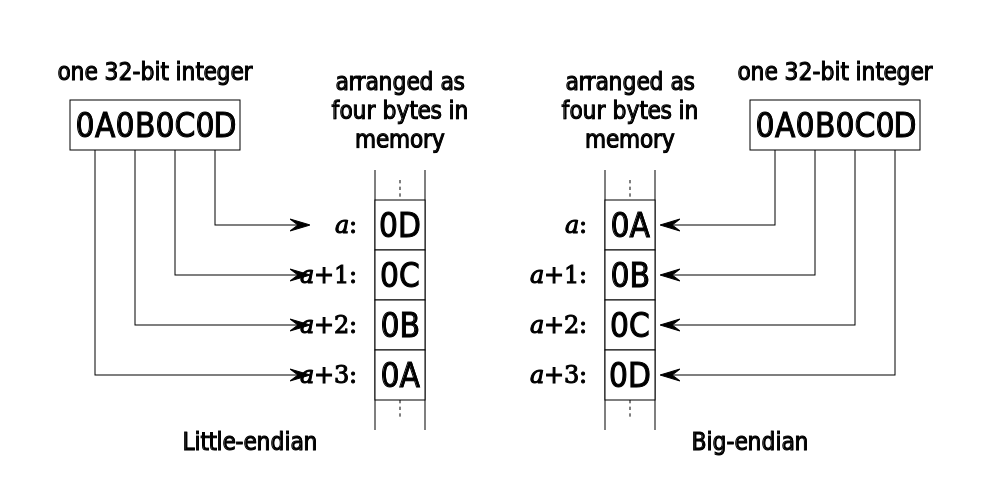
\includegraphics[width=0.8\textwidth]{figure/32bit-Endianess.png}
\end{figure}

\subsubsection{Logical Operations}

There are two types of logical shifts: arithmetic shifts and logical shifts. In an arithmetic shift, the sign bit is copied to the left during a right shift, while in a logical shift, the sign bit is always 0.

\begin{table}[H]
	\centering
	\begin{tabular}{lll}
		\toprule
		\textbf{Operation} & \textbf{Before} & \textbf{After} \\
		\midrule
		Logical Shift Right & 1001 & 0100 \\
		Arithmetic Shift Right & 1001 & 1100 \\
		\bottomrule
	\end{tabular}
\end{table}

\section{RISC-V Procedure}

\subsection{Procedure Call}

When a procedure is called, the following steps are taken:

\begin{table}[H]
	\centering
	\resizebox{\linewidth}{!}{
		\begin{tabular}{ll}
			\toprule
			\textbf{Step} & \textbf{Implementation} \\
			\midrule
			Put parameters in a place where the callee can access them & Typically in registers \texttt{a0} to \texttt{a7} \\
			Transfer control to the callee & Using the \texttt{jal} instruction \\
			Acquire the storage needed for the callee & Typically by decrementing the stack pointer \\
			Perform the desired task & \\
			Place the result in a place where the caller can access it & Typically in register \texttt{a0} - \texttt{a1} \\
			Return control to the caller & Using the \texttt{jalr} instruction \\
			\bottomrule
		\end{tabular}
	}
\end{table}

\subsection{Calling Convention}

The registers in RISC-V are divided into two categories: caller-saved registers and callee-saved registers. The difference here is that if the callee modifies a callee-saved register, it must restore the original value before returning control to the caller. But for caller-saved registers, the callee can modify them freely.

In convention, callee should save the following registers: \texttt{sp} (stack pointer) and \texttt{s0} to \texttt{s11} (saved registers).

\section{RISC-V Instruction Format}

\begin{table}[H]
	\centering
	\resizebox{\linewidth}{!}{
		\begin{tabular}{lll}
			\toprule
			\textbf{Type} & \textbf{Format} & \textbf{Feature} \\
			\midrule
			R-type & \texttt{funct7 rs2 rs1 funct3 rd opcode} & Take input from two registers and writes to one register \\
			I-type & \texttt{imm[11:0] rs1 funct3 rd opcode} & Involves an immediate value, might be arithmetic or load operation \\
			S-type & \texttt{imm[11:5] rs2 rs1 funct3 imm[4:0] opcode} & Store operation \\
			B-type & \texttt{imm[12] imm[10:5] rs2 rs1 funct3 imm[4:1] imm[11] opcode} & Branch operation \\
			U-type & \texttt{imm[31:12] rd opcode} & Load upper immediate \\
			J-type & \texttt{imm[20] imm[10:1] imm[11] imm[19:12] rd opcode} & Jump operation \\
			\bottomrule
		\end{tabular}
	}
\end{table}

\textit{Note:} The immediate value for B-type and J-type instructions needs to be left-shifted by 1 bit, while the immediate value for U-type instructions needs to be left-shifted by 12 bits.

\begin{tipsbox}
	\texttt{jalr} instruction is usually used to return from a procedure call. But it can also be used to jump to a far away address. For example, to jump to any 32-bit address, we can use the following code:
	\begin{verbatim}
		lui x1, <upper 20 bits>
		jalr x0, x1, <lower 12 bits>
	\end{verbatim}

	If we want to jump to PC-relative address with 32-bit offset, we simply replace the \texttt{lui} instruction above with \texttt{auipc} instruction:
	\begin{verbatim}
		auipc x1, <upper 20 bits>
		jalr x0, x1, <lower 12 bits>
	\end{verbatim}
\end{tipsbox}

\section{Performance}

\subsection{Performance Metrics}

There are two main performance metrics: response time and throughput. Response time is the time it takes to complete a task, while throughput is the number of tasks completed per unit time.

However, response time is not a good metric for performance evaluation because it includes all aspects of the system, such as the CPU, memory, and I/O devices. Instead, we usually use CPU time to evaluate the performance of a system, which is the time the CPU spends executing a task, excluding I/O time and other jobs' share.

\subsection{CPU Time}

To calculate the CPU time, we use the following formula:
\begin{equation*}
	\text{CPU time} = \frac{\text{CPU clock cycles}}{\text{Clock rate}} = \frac{\text{Instruction Count} \times \text{CPI}}{\text{Clock rate}}
\end{equation*}

The performance depends on the following factors:
\begin{table}[H]
	\centering
	\begin{tabular}{llll}
		\toprule
		\textbf{Component} & \textbf{IC} & \textbf{CPI} & \textbf{Clock Rate} \\
		\midrule
		Algorithm & Yes & Possible & No \\
		Programming Language & Yes & Yes & No \\
		Compiler & Yes & Yes & No \\
		Instruction Set Architecture & Yes & Yes & Yes \\
		\bottomrule
	\end{tabular}	
\end{table}

\section{Arithmetic}

\subsection{Addition and Subtraction}

Addition overflows when the sum of two positive numbers is negative or the sum of two negative numbers is positive. Subtraction overflows when the difference of a positive number and a negative number is negative or the difference of a negative number and a positive number is positive.

\paragraph{Saturating Arithmetic} In saturating arithmetic, the result is set to the maximum or minimum value when an overflow occurs.

\subsection{Multiplication}

A primitive multiplier for $n$-bit numbers consists of a $2n$-bit ALU, a $2n$-bit register for the multiplicand, a $2n$-bit register for the product, and an $n$-bit register for the multiplier. The procedure is as follows:
\begin{enumerate}
	\item Initialize the registers accordingly.
	\item If the least significant bit of the multiplier is 1, add the multiplicand to the product.
	\item Shift the product left by 1 bit.
	\item Shift the multiplier right by 1 bit.
	\item Repeat steps 2 to 4 for $n$ iterations.
	\item The product register contains the result.
\end{enumerate}

Here is an example of multiplying 2 by 7:
\begin{table}[H]
	\centering
	\begin{tabular}{lllll}
		\toprule
		\textbf{Iteration} & \textbf{Multiplier} & \textbf{Multiplicand} & \textbf{Product} & \textbf{Operation} \\
		\midrule
		0 & 0111 & 0000\_0010 & 0000\_0000 & Initialization \\
		\midrule
		\multirow{2}{*}{1} & 0111 & 0000\_0010 & 0000\_0010 & Add multiplicand \\
		& 0011 & 0000\_0100 & 0000\_0010 & Shift registers \\
		\midrule
		\multirow{2}{*}{2} & 0011 & 0000\_0100 & 0000\_0110 & Add multiplicand \\
		& 0001 & 0000\_1000 & 0000\_0110 & Shift registers \\
		\midrule
		\multirow{2}{*}{3} & 0001 & 0000\_1000 & 0000\_1110 & Add multiplicand \\
		& 0000 & 0001\_0000 & 0000\_1110 & Shift registers \\
		\midrule
		4 & 0000 & 0010\_0000 & 0000\_1110 & Shift registers \\
		\bottomrule
	\end{tabular}
\end{table}

An optimized multiplier for $n$-bit numbers consists of an $n$-bit ALU, an $n$-bit register for the multiplicand, and a $2n$-bit register for the product. The procedure is as follows:
\begin{enumerate}
	\item Initialize the multiplicand register with the multiplier. Initialize the product register's lower $n$ bits with multiplier and the upper $n$ bits with 0.
	\item If the least significant bit of the product register is 1, add the multiplicand to upper $n$ bits of the product register.
	\item Shift the product register right by 1 bit.
	\item Repeat steps 2 and 3 for $n$ iterations.
	\item The product register contains the result.
\end{enumerate}

Here is an example of multiplying 2 by 7:
\begin{table}[H]
	\centering
	\begin{tabular}{llll}
		\toprule
		\textbf{Iteration} & \textbf{Multiplicand} & \textbf{Product} & \textbf{Operation} \\
		\midrule
		0 & 0010 & 0000\_0111 & Initialization \\
		\midrule
		\multirow{2}{*}{1} & 0010 & 0010\_0111 & Add multiplicand \\
		& 0010 & 0001\_0011 & Shift right \\
		\midrule
		\multirow{2}{*}{2} & 0010 & 0011\_0011 & Add multiplicand \\
		& 0010 & 0001\_1001 & Shift right \\
		\midrule
		\multirow{2}{*}{3} & 0010 & 0011\_1001 & Add multiplicand \\
		& 0010 & 0001\_1100 & Shift right \\
		\midrule
		4 & 0010 & 0000\_1110 & Shift right \\
		\bottomrule
	\end{tabular}
\end{table}

\subsection{Division}

A primitive divider for $n$-bit numbers consists of a $2n$-bit ALU, a $2n$-bit register for the divisor, a $2n$-bit register for the remainder, and an $n$-bit register for the quotient. The procedure is as follows:
\begin{enumerate}
	\item Initialize the divisor register's upper $n$ bits with the divisor and the lower $n$ bits with 0. Initialize the remainder register's lower $n$ bits with the dividend and the upper $n$ bits with 0. Initialize the quotient register with 0.
	\item Subtract the divisor from the remainder.
	\item If the result is negative, add the divisor back to the remainder. Shift the quotient left by 1 bit and add 0 to the least significant bit. Else, shift the quotient left by 1 bit and add 1 to the least significant bit.
	\item Shift the divisor right by 1 bit.
	\item Repeat steps 2 to 4 for $n+1$ iterations.
	\item The quotient register contains the quotient, and the remainder register contains the remainder.
\end{enumerate}

Here is an example of dividing 7 by 2:
\begin{table}[H]
	\centering
	\begin{tabular}{lllll}
		\toprule
		\textbf{Iteration} & \textbf{Divisor} & \textbf{Remainder} & \textbf{Quotient} & \textbf{Operation} \\
		\midrule
		0 & 0010\_0000 & 0000\_0111 & 0000 & Initialization \\
		\midrule
		\multirow{3}{*}{1} & 0010\_0000 & 1110\_0111 & 0000 & Subtract divisor \\
		& 0010\_0000 & 0000\_0111 & 0000 & Restore \\
		& 0001\_0000 & 0000\_0000 & 0000 & Shift registers \\
		\midrule
		\multirow{3}{*}{2} & 0001\_0000 & 1111\_0111 & 0000 & Subtract divisor \\
		& 0001\_0000 & 0000\_0111 & 0000 & Restore \\
		& 0000\_1000 & 0000\_0000 & 0000 & Shift registers \\
		\midrule
		\multirow{3}{*}{3} & 0000\_1000 & 1111\_1111 & 0000 & Subtract divisor \\
		& 0000\_1000 & 0000\_0111 & 0000 & Restore \\
		& 0000\_0100 & 0000\_0000 & 0000 & Shift registers \\
		\midrule
		\multirow{3}{*}{4} & 0000\_0100 & 0000\_0011 & 0000 & Subtract divisor \\
		& 0000\_0010 & 0000\_0011 & 0000 & Shift registers \\
		& 0000\_0010 & 0000\_0011 & 0001 & Add 1 to quotient \\
		\midrule
		\multirow{3}{*}{5} & 0000\_0010 & 0000\_0001 & 0001 & Subtract divisor \\
		& 0000\_0001 & 0000\_0001 & 0010 & Shift registers \\
		& 0000\_0001 & 0000\_0001 & 0011 & Add 1 to quotient \\
		\bottomrule
	\end{tabular}
\end{table}

An optimized divider for $n$-bit numbers consists of an $n$-bit ALU, an $n$-bit register for the divisor, and a $2n$-bit register for the remainder. The procedure is as follows:
\begin{enumerate}
	\item Initialize the divisor register with the divisor. Initialize the lower $n$ bits of the remainder register with the dividend and the upper $n$ bits with 0.
	\item Shift the remainder register left by 1 bit.
	\item Subtract the upper $n$ bits of the remainder register from the divisor.
	\item If the result is negative, add the divisor back to the upper $n$ bits of the remainder register, else add 1 to the lower $n$ bits of the remainder register.
	\item Repeat steps 2 to 4 for $n$ iterations.
	\item The lower $n$ bits of the remainder register contain the quotient, and the upper $n$ bits contain the remainder.
\end{enumerate}

Here is an example of dividing 7 by 2:
\begin{table}[H]
	\centering
	\begin{tabular}{llll}
		\toprule
		\textbf{Iteration} & \textbf{Divisor} & \textbf{Remainder} & \textbf{Operation} \\
		\midrule
		0 & 0010 & 0000\_0111 & Initialization \\
		\midrule
		\multirow{2}{*}{1} & 0010 & 0000\_1110 & Shift left \\
		& 0010 & 1110\_1110 & Subtract divisor \\
		& 0010 & 0000\_1110 & Restore \\
		\midrule
		\multirow{2}{*}{2} & 0010 & 0001\_1100 & Shift left \\
		& 0010 & 1111\_1100 & Subtract divisor \\
		& 0010 & 0001\_1100 & Restore \\
		\midrule
		\multirow{2}{*}{3} & 0010 & 0011\_1000 & Shift left \\
		& 0010 & 0001\_1000 & Subtract divisor \\
		& 0010 & 0001\_1001 & Add 1 \\
		\midrule
		\multirow{2}{*}{4} & 0010 & 0011\_0010 & Shift left \\
		& 0010 & 0001\_0010 & Subtract divisor \\
		& 0010 & 0001\_0011 & Add 1 \\
		\bottomrule
	\end{tabular}
\end{table}

\paragraph{Sign Convention} In signed division, the sign of the quotient is negative if and only if the signs of the dividend and divisor are different. The remainder has the same sign as the dividend. For example, $-7 \div 2 = -3 \dots -1$.

\section{Floating Point Arithmetic}

\subsection{Floating Point Representation}

A floating point number consists of three parts: the sign bit, the exponent, and the fraction (mantissa). The value of the number is:
\begin{equation*}
	(-1)^s \times 2^{e - B} \times 1.f
\end{equation*}
where $s$ is the sign bit, $e$ is the exponent, $B$ is the bias, and $f$ is the fraction.

\paragraph{Bias} The bias is calculated as $2^{k-1} - 1$, where $k$ is the number of bits used to represent the exponent. The purpose of the bias is to treat the exponent as an unsigned number.

\paragraph{Relative Precision} The relative precision is $2^{-f}$, where $f$ is the number of bits used to represent the fraction. To convert the relative precision to the number of decimal places, we use the formula $-\log_{10}(2^{-f}) = f \times \log_{10}2$.

\subsection{Floating Point Special Encoding}

There are three special encodings for floating point numbers: zero, infinity, and NaN (Not a Number). Zero is represented by all bits being 0, infinity is represented by the exponent being all 1s and the fraction being 0, and NaN is represented by the exponent being all 1s and the fraction being non-zero. To be noticed, there are two types of infinity: positive and negative (determined by the sign bit).

There is also a denormalized representation for floating point numbers. In this representation, the exponent is 0, and the fraction is non-zero. The value of the number is:
\begin{equation*}
	(-1)^s \times 2^{1 - B} \times 0.f
\end{equation*}

The overall representation of floating point numbers is as follows:
\begin{table}[H]
	\centering
	\begin{tabular}{lll}
		\toprule
		\textbf{Exponent} & \textbf{Fraction = 0} & \textbf{Fraction $\neq$ 0}\\
		\midrule
		0 & $\pm 0$ & Denormalized \\
		1 to $2^k - 2$ & Normalized & Normalized \\
		$2^k - 1$ & $\pm \infty$ & NaN \\
		\bottomrule
	\end{tabular}
\end{table}

\begin{warningbox}
	When calculating the range of a normalized floating point number, we need to be careful with the exponent. The minimum exponent is 1, and the maximum exponent is $2^k - 2$. 0 and $2^k - 1$ are reserved for special encodings.
\end{warningbox}

\subsection{Floating Point Arithmetic}

The procedure for floating point addition and subtraction is as follows:
\begin{enumerate}
	\item Align the exponents of the two numbers, the final exponent is the larger of the two exponents.
	\item Add or subtract the significands of the two numbers.
	\item Normalize the result (shift the significand until $1 \leq |f| < 2$).
	\item Round the result (and renormalize if necessary).
\end{enumerate}

The procedure for floating point multiplication is as follows:
\begin{enumerate}
	\item Add the exponents of the two numbers.
	\item Multiply the significands of the two numbers.
	\item Normalize the result (shift the significand until $1 \leq |f| < 2$).
	\item Round the result (and renormalize if necessary).
	\item Determine the sign of the result.
\end{enumerate}

\section{Pipeline}

\subsection{Inefficiency of Single Cycle CPU}

In a single cycle CPU, the clock cycle is determined by the slowest instruction (the longest delay). This means most module will be idle for most of the time, which is inefficient.

\subsection{Pipeline Performance}
\label{sec:pipeline-performance}

Suppose all stages are balanced, the speedup of a pipeline is given by:
\begin{equation*}
	\text{Clock Cycle Time}_{\text{pipelined}} = \frac{\text{Clock Cycle Time}_{\text{non-pipelined}}}{\text{Number of Stages}}
\end{equation*}

To be noticed that the latency (time to complete a single instruction) of a pipelined CPU will not be reduced. In fact, the latency may increase especially when stages are not balanced. Pipeline is more about throughput (number of instructions completed per unit time) than latency.

\subsection{Pipeline Hazards}

There are three types of pipeline hazards: structural hazards, data hazards, and control hazards.
\begin{itemize}
	\item Structural hazards: Two instructions require the same hardware resource.
	\item Data hazards: The next instruction to execute requires the result of the current instruction.
	\item Control hazards: Which instruction to execute next is determined by the result of the current instruction.
\end{itemize}

The structure hazards do not occur in RISC-V, because the ISA is designed under Harvard architecture (separate instruction and data memory). This avoids the conflict between instruction fetch and data access. The two other hazards, however, still exist.

\subsubsection{Data Hazards}

Generally, we solve data hazards by either stalling the pipeline or forwarding the data, sometimes a combination of both.

\paragraph{Stall Only} When stalling the pipeline, we insert a no-operation (NOP) instruction to the pipeline. This is the simplest way to solve data hazards, but it is also the least efficient.

\paragraph{Forwarding Only} We add extra data path to forward the data from the output of the ALU (or memory) to the input of the ALU. Forwarding data from ALU to ALU is called EX-EX forwarding (or ALU-ALU forwarding), while forwarding data from memory to ALU is called MEM-EX forwarding (or MEM-ALU forwarding). However, this method is not always applicable (cannot handle load-use hazards).

\paragraph{Stall and Forwarding} We stall the pipeline only when forwarding is not possible (load-use hazards), which requires more modules for hazard detection and control.

\begin{figure}[H]
	\centering
	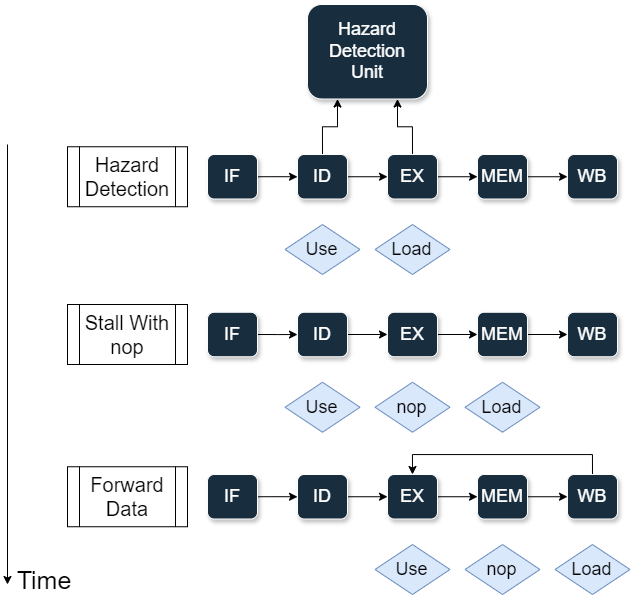
\includegraphics[width=0.8\textwidth]{figure/Hazard Detection.png}
	\caption{Stall and Forwarding for Load-Use Hazards}
\end{figure}

\subsubsection{Control Hazards}

Generally, we solve control hazards by stalling and flushing the pipeline. When a branch instruction is detected, we stall the pipeline (by inserting NOPs or filling the pipeline with predicted instructions). After we know the result of the branch instruction, we can check if the prediction is correct. If it is not, we flush the pipeline (discard the instructions after the branch instruction) and restart the pipeline.

If extra hardware is available, we can determine the branch target early in the instruction decode stage and reduce the number of stalls.

\paragraph{Static and Dynamic Branch Prediction} In static branch prediction, the prediction is made at compile time by the compiler. In dynamic branch prediction, the prediction is made at run time by looking at the history of the branch instruction.

\section{Instruction-Level Parallelism}

\subsection{Deeper Pipeline}

If we further break down the process and hence have more stages in the pipeline, we can achieve shorter clock cycle time (please refer to Section \ref{sec:pipeline-performance}). 

\subsection{Multiple Issue}

Multiple issue means execute multiple instructions in parallel in a single clock cycle (This may cause CPI to be less than 1. If so we use IPC, Instructions Per Cycle). The key procedure of multiple issue is to resolve instruction dependencies and pack instructions into issue packets.

\subsubsection{Static Multiple Issue}

In static multiple issue, compilers is responsible for reordering the instructions to avoid hazards. This is also called Very Long Instruction Word (VLIW) architecture. 

\paragraph{Data Dependencies} It is obvious that two instructions that one depends on the other cannot be issued in parallel. For example, a load instruction that requires the address calculated by the previous instruction.

\paragraph{Hardware Race} The critical problem for hardware is that the data memory can only be accessed once in a clock cycle. Hence, two instructions that both require data memory access cannot be issued in parallel. This is why the issue packet is designed to have one slot for ALU / Branch instruction (which does not require data memory access) and one slot for Load / Store instruction (which requires data memory access).  

\begin{examplebox}
	For this loop assembly code:
	\begin{verbatim}
		lw   t0, 0(s1)          // s1 is pointer to the array
		add  t0, t0, s2         // add a constant to the array element
		sw   t0, 0(s1)          // store the result back to the array
		addi s1, s1, -4         // move to the next element
		bge  s1, zero, loop     // loop back
	\end{verbatim}
	The optimal reordering for an 2-issue processor will have an IPC of 1.25:
	\begin{verbatim}
		ALU / Branch            Load / Store
		nop                     lw  t0, 0(s1)
		addi s1, s1, -4         nop
		add  t0, t0, s2         nop
		bge  s1, zero, loop     sw  t0, 0(s1)
	\end{verbatim}
	To be noticed that the \texttt{add} and \texttt{addi} instructions cannot swap their positions, otherwise it will cause a load-use hazard.
\end{examplebox}

\paragraph{Loop Unrolling} One technique to resolve name dependencies is Loop Unrolling. For example, if we have a loop that loads an element from an array, perform some operations, and store the result back to the array, and the loop is executed for 4 times. This loop cannot be issued in parallel because the loop body use the same register and every instruction depends on this register. This is so-called name dependencies, because the dependencies is not caused by data but reusing register name. To resolve this, we can unroll the loop, which means we copy the loop body 4 times and change the register name for each copy. This way, the instructions in different loop bodies can be issued in parallel.

\begin{verbatim}
	// Original Loop
	for (int i = 0; i < 4; i++) {
	    A[i] = A[i] + 1; // use the same register to hold A[i]
	}

	// Unrolled Loop
	A[0] = A[0] + 1; // use different register for A[0], A[1], A[2], A[3]
	A[1] = A[1] + 1;
	A[2] = A[2] + 1;
	A[3] = A[3] + 1;
\end{verbatim}

\subsubsection{Dynamic Multiple Issue}

In dynamic multiple issue, the CPU examines the instruction stream and decides which instructions to execute in parallel. This is also called ``Superscalar'' architecture.

\paragraph{Out-of-Order Execution} In out-of-order execution, the CPU executes the instructions in the order that minimizes the pipeline stalls. It Involves three steps: in-order issue: issue the instructions to the reservation station in order; out-of-order execution: execute the instructions in the reservation station whenever the operands are ready; in-order commit: commit the instructions in order to the register file.

\subsection{Speculative Execution}

In speculative execution, the CPU executes the instructions before it knows whether they should be executed. This is used to reduce the branch penalty. Additionally, this helps load cache data before it is needed.

\subsection{Register Renaming}

Register renaming is used to resolve the name dependencies. The CPU uses a physical register file to store the data, and a mapping table to map the logical register to the physical register. This way, the CPU can issue the instructions in parallel even if they use the same logical register.

\section{Memory Hierarchy}

\subsection{Cache}

\subsubsection{Direct Mapped Cache}

In a direct mapped cache, each memory block can only be stored in one specific cache block. The cache block is determined by the lower bits of the memory block address. The cache block consists of the tag, the index, the valid bit, and the data, and the number of bits in each part is calculated as follows:
\begin{align*}
	\#\text{Offset bits} &= \log_2(\text{Block Size}) \\
	\#\text{Index bits} &= \log_2(\text{Number of Blocks}) \\
	\#\text{Tag bits} &= \text{Address bits} - \text{Offset bits} - \text{Index bits}
\end{align*}

\begin{warningbox}
	For fixed-sized cache, increasing the block size may not necessarily reduce the miss rate. This is because the larger block size will decrease the number of blocks in the cache, which may lead to more conflicts. Also, the larger block size will increase the miss penalty (the time to load a block from memory to cache).
\end{warningbox}

\subsubsection{Set Associative Cache}

In a set associative cache, several cache blocks are mapped to the same set. Each memory block can only be stored in one of the cache set but can be stored in any block within the set. The cache block consists of the tag, the index (set), the valid bit, and the data, and the number of bits in each part is calculated as follows:
\begin{align*}
	\#\text{Offset bits} &= \log_2(\text{Block Size}) \\
	\#\text{Index bits} &= \log_2(\text{Number of Sets}) \\
	\#\text{Tag bits} &= \text{Address bits} - \text{Offset bits} - \text{Index bits}
\end{align*}

\subsubsection{Fully Associative Cache}

In a fully associative cache, each memory block can be stored in any cache block. The cache block consists of the tag, the valid bit, and the data, and the number of bits in each part is calculated as follows:
\begin{align*}
	\#\text{Offset bits} &= \log_2(\text{Block Size}) \\
	\#\text{Tag bits} &= \text{Address bits} - \text{Offset bits}
\end{align*}

\subsubsection{Multi-Level Cache}

In a multi-level cache, we put the L1 cache (smaller but faster) closer to the CPU and the L2 cache (larger but slower) further away. This layout effectively reduces the miss rate.

\begin{tipsbox}
	The overall storage system can be viewed as a huge multi-level cache, consisting of the CPU registers, the L1 cache, the L2 cache, the main memory, and the disk. The closer the storage is to the CPU, the faster but smaller it is.
\end{tipsbox}

\subsubsection{Pros and Cons of Different Cache}

Generally, the higher the associativity, the lower the miss rate. However, to achieve higher associativity, we need more hardware (comparators, etc.), which increases the cost of the cache and the access time. 

\subsection{Cache Miss}

There are three types of cache miss: compulsory miss, capacity miss, and conflict miss.
\begin{itemize}
	\item Compulsory miss: On startup, the cache is empty, so the first access to a memory block will always miss.
	\item Capacity miss: The cache is full. Hence, any new memory block must replace an existing block.
	\item Conflict miss: Although the cache is not full, the memory block cannot be stored in the cache because of the block (or set) it maps to is already occupied (only for set associative or direct mapped cache).
\end{itemize}

We can optimize the cache design to reduce the miss rate. Below are some common trade-offs:
\begin{table}[H]
	\centering
	\begin{tabular}{lll}
		\toprule
		\textbf{Trade-off} & \textbf{Pros} & \textbf{Cons} \\
		\midrule
		Increase cache size & Reduce capacity miss & Higher access time \\
		Increase associativity & Reduce conflict miss & Higher access time and extra hardware \\
		Increase block size & Reduce compulsory miss & Higher miss penalty \\
		\bottomrule
	\end{tabular}
\end{table}

\subsection{Write Policy}

On write hit (the memory block we want to write is already in the cache), we can use write-through or write-back policy.
\begin{itemize}
	\item Write-through: The data is written to both the cache and the memory. This is simpler but slower.
	\item Write-back: The data is written to the cache only. The data in the memory is updated only when the cache block is replaced. This is faster but more complex and require an extra dirty bit (to indicate whether the cache block is modified) for each cache block.
\end{itemize}

On write miss (the memory block we want to write is not in the cache), we can use write-allocate or write-around policy.
\begin{itemize}
	\item Write-allocate: The memory block is loaded into the cache and then the data is written to the cache.
	\item Write-around: The data is written to the memory only. The cache is not updated.
\end{itemize}

\subsection{Cache Performance}

The cache performance is evaluated by Average Memory Access Time (AMAT), which is calculated as follows:
\begin{equation*}
	\text{AMAT} = \text{Hit Time} + \text{Miss Rate} \times \text{Miss Penalty}
\end{equation*}

For multi-level cache, the miss rate is divided into each level, and sometimes calculated within the level (local miss rate) or globally (global miss rate). The difference is shown as follows:
\begin{align*}
	\text{Global Miss Rate for level}_i &= \frac{\text{Total number of misses on level}_i}{\text{Total number of block requests}} \\
	\text{Local Miss Rate for level}_i &= \frac{\text{Number of misses on level}_i}{\text{Number of block requests on level}_i}
\end{align*}

The AMAT for multi-level cache is calculated by using the global miss rate:
\begin{align*}
	\text{AMAT} &= \text{L1 Hit Time} \\
	&+ \text{L1 Global Miss Rate} \times \text{L1 Miss Penalty} \\
	&+ \text{L2 Global Miss Rate} \times \text{L2 Miss Penalty}
\end{align*}
or by using the local miss rate:
\begin{align*}
	\text{AMAT} &= \text{L1 Hit Time} \\
	&+ \text{L1 Local Miss Rate} \\
	&\times \left( \text{L1 Miss Penalty} + \text{L2 Local Miss Rate} \times \text{L2 Miss Penalty} \right)
\end{align*}

\subsection{Dependability Measures}

There are three metrics to evaluate the dependability of a cache: mean time to failure (MTTF), mean time to repair (MTTR), and availability. The availability is calculated as follows:
\begin{equation*}
	\text{Availability} = \frac{\text{MTTF}}{\text{MTTF} + \text{MTTR}}
\end{equation*}

\subsection{Error Detection and Correction}

\subsubsection{Hamming Distance}

The Hamming distance is the minimum number of bit flips required to convert one valid pattern to another. 

For Hamming distance $d = 2$, this allows single-bit error detection. For Hamming distance $d = 3$, this allows single-bit error correction. The difference is caused by some points that are equidistant to two valid patterns.

\subsubsection{Hamming Code}

In this course, we only consider SEC / DED codes (Single Error Correction / Double Error Detection), where Hamming Code is the most common example. The Hamming Code is constructed as follows:
\begin{enumerate}
	\item Determine the number of parity bits required by the formula $2^p \geq m + p + 1$, where $m$ is the number of data bits and $p$ is the number of parity bits.
	\item The positions of the parity bits are determined by the power of 2 (1, 2, 4, 8, etc.), and each parity bit is named by its position ($p_1, p_2, p_4, p_8, \ldots$).
	\item Let the parity bit $p_{2^i}$ checks the parity of the bits where the $i$-th bit is 1 (including itself). The overall parity should be even.
\end{enumerate}

To detect and correct errors, we can use the following steps:
\begin{enumerate}
	\item Calculate the parity bits using the data bits.
	\item Compare the calculated parity bits with the received parity bits.
	\item If the parity bits are different, there is an error. The position of the error is determined by the sum of subscript of the parity bits that are different. For example, if $p_1$ and $p_4$ are different, the error is at the 5-th bit.
\end{enumerate}

\paragraph{Double Error Detection} To detect double errors, we can add an extra parity bit $p_n$ that checks the parity of all bits. If there is only one error, $p_n$ will be incorrect. If there are two errors, $p_n$ will still be correct, but some other parity bits will be incorrect.

\subsection{Virtual Memory}

\subsubsection{Page Table}

Sometimes we increase the address space by using virtual memory, with some parts stored in the disk. Hence, before accessing the memory, we need to translate the virtual address to the physical address. The translation is done with the help of the page table.

The page table contains all mappings from virtual pages to physical pages. Hence, there is no index bit in the page table, because the virtual page number is the index. The page table consists of the valid bit and the physical page number.

\subsubsection{Translation Look-aside Buffer (TLB)}

Since page table needs to hold all mappings, it is large and can only be stored in the main memory. However, main memory access is slow. To speed up the translation, we use TLB, which is a small cache for the page table. 

Since the TLB is essentially a cache, the structure is the same as the previous section mentioned, and we will not repeat it here.

\subsection{Overall Memory Hierarchy}

When fetching data, we go through the following steps:
\begin{enumerate}
	\item Translate the virtual address to the physical address.
	\begin{enumerate}
		\item Check TLB. If the translation is in the TLB, use the physical page number directly. Else, go to the next step.
		\item Access the page table in the main memory. If the physical page number is located on disk, raise a page fault. Else, use the physical page number.
	\end{enumerate}
	\item Access the cache. If the data is in the cache, use the data directly. Else, go to the next step.
	\item Access the main memory. 
\end{enumerate}

\begin{warningbox}
	There are two scenarios that will never happen:
	\begin{enumerate}
		\item We miss both the TLB and page table but hit the cache (or memory): Unless a page fault occurs, the data must be in the cache or memory.
		\item We hit TLB but miss the page table: Since the TLB is a cache for the page table, and page table is the only source for the physical page number.
	\end{enumerate}
	\textit{Note:} TLB miss here means the page we required is not in memory, not we cannot find the virtual page number in TLB (which is impossible).
\end{warningbox}

\section{Parallel Processor}

The goal of parallel processor is to replace large inefficient processors with multiple smaller processors, which improves scalability, availability and power efficiency. 

Parallelism can be achieved in multiple ways:
\begin{itemize}
	\item Task-level parallelism: execute independent jobs in parallel.
	\item Parallel processing program: One program that utilize multiple processors.
	\item Multicore processor: Multiple processors on a single chip.
\end{itemize}

However, the challenge of parallelism comes from both hardware and software. The hardware challenge is that serial hardware is much simpler than parallel hardware. The software challenge is sequential program is much easier to write and debug than concurrent program.

\subsection{Amdahl's Law}

Amdahl's Law is used to evaluate the speedup of a program when parallelized. The speedup is calculated as follows:
\begin{equation*}
	\text{Speedup} = \frac{1}{(1 - f) + \frac{f}{n}}
\end{equation*}
where $f$ is the fraction of the program that can be parallelized and $n$ is the number of processors.

The maximum speedup is given by:
\begin{equation*}
	\lim_{n \to \infty} \text{Speedup} = \frac{1}{1 - f}
\end{equation*}

Amdahl's law tells us we can never achieve reverse proportional speedup by adding more processors, due to the presence of the serial part of the program, as the maximum speedup is $\frac{1}{1 - f}$.

\begin{tipsbox}
	How Amdahl's Law is derived:
	\begin{align*}
		\text{Speedup} &= \frac{T_{\text{old}}}{T_{\text{new}}} \\
		&= \frac{T_{\text{old}}}{(1 - f) \times T_{\text{old}} + \frac{f \times T_{\text{old}}}{n}} \\
		&= \frac{1}{(1 - f) + \frac{f}{n}}
	\end{align*}
\end{tipsbox}

\paragraph{Strong and Weak Scalability} Strong scalability is that if the problem size is fixed, the time should be reversed proportional to the number of processors. Weak scalability is that if the number of processors is proportional to the problem size, the time should be constant. Weak scalability is more common in practice and strong scalability is more difficult to achieve, due to Amdahl's Law.

\subsection{Single Instruction Multiple Data (SIMD)}

In SIMD, processor operates on a vector of data with a single instruction. Or, all processors execute the same instruction, but each with different data address. This is a simple way to achieve synchronization.

\subsection{Multithreading}

In multithreading, processor can switch between different threads to achieve parallelism. When one thread is stalled, the processor can switch to another thread. There are two types of multithreading: fine-grained multithreading (switch between threads in every cycle) and coarse-grained multithreading(switch only on long stalls, such as cache miss).

\paragraph{Simultaneous Multithreading (SMT)} In SMT, the processor can execute multiple threads simultaneously. This is achieved by multiple-issue processor. SMT utilize resources more efficiently than the two types of multithreading mentioned above. In traditional multithreading, only one thread can use the resources at a time. This usually cannot fully utilize all issue slots in the processor. In SMT, the vacant resources can be used by another thread.

\subsection{Shared Memory Multiprocessor}

In shared memory multiprocessor, all processors share the same memory. Hence, if one program is written into the memory, all processors can read it. 

\subsection{Message Parsing Multiprocessor}

In message parsing multiprocessor, each processor has its own memory. The processors communicate with each other by sending messages. This is more scalable than shared memory multiprocessor, but the communication is more complex.
\end{document}